%! TeX root = ../charles/en/thesis.tex
\chapter{Method and Setup}
\label{chap:setup}

We continue training the Merlot Reserve~\citep{zellers2022mreserve} model on
videos from the Charades dataset~\citep{sigurdsson2016charades}. We call this
process post-pretraining, rather than finetuning, since the objective function
is very similar to the pre-training stage, but we train on a smaller dataset
that is designed to improve the temporal reasoning of the Merlot Reserve model
before being evaluated on downstream tasks. This chapter explains the creation
process of this new dataset, as well as the post-pretraining process.

\section{Dataset Creation}
\label{sec:data}

We use videos and annotations from Charades to create our new dataset. This is
motivated by the desire to have videos annotated with descriptive actions,
while also having annotated timespans associated with the actions that allows
for creating segments that are well aligned with frames presented to the model.
From these actions and timespans, we are able to create text labels that
describe a variety of temporal relations between a pair of actions.

Since one of our evaluation benchmarks, STAR~\citep{wu2021star}, uses the same
dataset as its video source, we filter video ids that appear in the validation
and test sets of STAR to avoid contamination of the evaluation data. We further
filter based on videos that contain at least 2 actions. This provides 7204
videos, annotated with actions and their timespans.

For each video, we create relation based on annotated actions. Each relation is
based on Allen's Interval Algebra~\citep{allen1983interval}, shown in Table
\ref{tab:allen_interval}. This simple calculus provides a powerful template for
reasoning about all types of temporal relation. By going beyond just before and
after, we are able to model actions that happen at any point in relation to one
another, providing a much more powerful schema.

The dataset is specifically designed to provide annotations that fit the
expected input for Merlot Reserve, but could trivially be generalised to work
with other models that use a masked language modelling objective.  That is, we
create aligned segments of frames, text, and audio per instance.  Using actions
and timestamps allows for a close alignment between frames and annotation,
which would not be possible if we were to use whole video descriptions.
Following Merlot Reserve, we use 8 segments per instance.

\begin{table}[tp]
	\centering
	\caption{The Thirteen Possible Relationships. All relation types except for
		\textit{equal} have a corresponding inverse relation type, which is
		used instead 50\% of the time. To create segments, three frames are
		selected based on the timespans of $X$ and $Y$. m($\cdot$), s($\cdot$),
		e($\cdot$), t($\cdot$) indicate the mid, start, end and one-third points of
	a timespan, respectively. Modified from~\citet{allen1983interval}.}
	\label{tab:allen_interval}
	\begin{tabular}{llc}
	\toprule
	Relation & Example & Frames Selected\\
	\midrule
	$X$ \textit{before} $Y$ & \texttt{XXX\space\space YYY} & [m($X$)~;~m(e($X$):s($Y$))~;~m($Y$)] \\
	$X$ \textit{meets} $Y$ & \texttt{XXXYYY} & [m($X$)~;~m(e($X$):s($Y$))~;~m($Y$)] \\
	$X$ \textit{overlaps} $Y$ & \texttt{XXX} & [t($X$)~;~m(e($X$):s($Y$))~;~2t($Y$)]\\
											& \texttt{\space YYY} & \\
	$X$ \textit{starts} $Y$ & \texttt{XXX} & [m($X$)~;~e($X$)~;~2t($Y$)]\\
										  & \texttt{YYYYY} & \\
	$X$ \textit{during} $Y$ & \texttt{\space XXX} & [s($Y$)~;~m($X$)~;~e($Y$)]\\
										  & \texttt{YYYYYY} & \\
	$X$ \textit{finishes} $Y$ & \texttt{\space\space XXX} & [t($Y$)~;~s($X$)~;~m($X$)] \\
											& \texttt{YYYYY} & \\
	$X$ \textit{equals} $Y$ & \texttt{XXX} & [m(s($X$):s($Y$))~;~m(m($X$):m($Y$))~;~m(e($X$):e($Y$))] \\
										  & \texttt{YYY} & \\
	\bottomrule
	\end{tabular}
\end{table}

\subsection{Creating Segments}
\label{ssec:create_segs}

For each video, we have relations between pairs of actions $X, Y$.  We create
instances for each relation, such that one instance contains annotations for a
relation between exactly two actions. We create up to $\binom{N}{2}$ instances
per video, where $N$ is the number of actions labeled in each video. The total
number of instances is 32627. An instance is made up of the label for action
$X$, a temporal expression $\tau$, and the label for action $Y$. Each action
pair has a timespan $(X_{start}, X_{end}), (Y_{start}, Y_{end})$ associated
with the action. $\tau$ is chosen based on these start and end times, according
to Allen's Interval Algebra, including a threshold of 1 second to define the
range of time that constitutes the difference between different relation types
\footnote{We find that 1 second provides a good compromise balance slight
inaccuracies in annotated time stamps while selecting the correct relation
type}. For example, if action $X$ has timespan (0.4, 6.7) and action $Y$ has
timespan (6.5, 10.0), this would create the instance $X$ \textit{meets} $Y$,
since the overlap between the end of $X$ and the start of $Y$ is less than the
threshold, and such a small overlap does not constitute creating an instance
with the relation type \textit{overlaps}.

Once the relation type for a pair of actions is identified, we create the
triple $(X,\tau,Y)$, split into three segments as follows. We split the label
into three, depending on the relation type, to create a complete annotation
that aims to match the average length of text spans from Merlot Reserve.

%We split the label into three
%\mbox{[$X$[:-1]~;~$X$[-1:]+$\tau$+$Y$[:1]~;~$Y$[1:]]}, where $X[:-1]$ indicates
%slicing up to the last word of action $X$, $[\cdot+\cdot]$ indicates
%concatenation, and $[\cdot~;~\cdot]$ indicates segment boundaries. This
%creates three segment labels roughly equal in length, with the temporal expression
%$\tau$ in the middle segment.

We then select frames and audio spectrograms based on timestamps. For the three
annotated segments, timestamps are chosen based on the relation type and action
timespans (see \cref{tab:allen_interval}). The other five timestamps are then
selected uniformly from either side of the annotations such that remaining
frames span the length of the whole video. Depending on when the actions occur
in the video, different numbers of timestamps will be taken from before and
after the annotated segments. Once we have eight timestamps corresponding to
the eight segments, we select one frame for each timestamp, and create audio
spectrograms following Merlot Reserve, with 5 second clips surrounding the
timestamp. If this causes an overlap with the timespan of another spectrogram,
the overlap is silenced, so as not to cause any information leakage that may
otherwise occur when predicting masked segments.

\subsection{Positive Labels}
\label{ssec:pos_labels}

Each segment is then made up of a frame, an audio spectrogram, and an
annotation.  The annotation may be empty, or may be one of the three segment
labels we create in~\cref{ssec:create_segs}. Since our temporal relation types
do not at this stage include inverse relations (we have a relation type before,
but not after), we map temporal relation types to temporal expressions with
50\% chance that the annotation is inverted, including inverting the order of
the actions. For example, if we have the triple (tidying up a blanket, \textit{before},
tidying something on the floor), this could create the segment labels [tidying
up a; blanket before tidying; something on the floor], or, if inverted,
[tidying something on the; floor after tidying; up a blanket]. This creates a
balance between opposite temporal relation types.

Mappings from temporal relation types to temporal expressions are shown in
\cref{tab:temp_maps}

\begin{table}[t]
	\centering
	\caption{Mappings from temporal relation types to temporal expressions and their inverses. For inverse temporal expressions, the order of actions \texttt{X} and \texttt{Y} is swapped. For \textit{starts} and \textit{finishes} relations, the final segment includes \texttt{Y} or \texttt{X} depending on whether a normal or inverse temporal expression is used, respectively.}
	\label{tab:temp_maps}
    \scriptsize
	\begin{tabular}{llll}
		\toprule
		Relation Type & Temporal Expression & Inverse Temporal Expression & Annotation \\
	\midrule
		\textit{before} & \texttt{before} & \texttt{after} & \texttt{[X;$\epsilon$;$\tau$+Y]}\\
			\textit{meets} & \texttt{immediately before} & \texttt{immediately after} & \texttt{[X[:-1];X[-1:]+$\tau$+Y[:1];Y[1:]]}\\
			\textit{overlaps} & \texttt{overlaps with} & \texttt{is overlapped by} & \texttt{[X[:-1];X[-1:]+$\tau$+Y[:1];Y[1:]]}\\
			\textit{starts} & \texttt{(at the same time as,} & \texttt{(at the same time as,} & \texttt{[X;$\tau$[0]+Y[:-1];}\\
							& \texttt{then continues)} & \texttt{then continues)} & \texttt{ Y[-1:]+$\tau$[1]+(Y$\mid$X)]}\\
			\textit{during} & \texttt{during} & \texttt{interrupted by} & \texttt{[X[:-1];X[-1:]+$\tau$+Y[:1];Y[1:]]}\\
			\textit{finishes} & \texttt{(before, while)} & \texttt{(while, after)} & \texttt{[Y;$\tau$[0]+X[:-1];}\\
							  & & & \texttt{ X[-1:]+$\tau$[1]+(X$\mid$Y)]}\\
			\textit{equals} & \texttt{and} & \texttt{and} & \texttt{[X[:-1];X[-1:]+$\tau$+Y[:1];Y[1:]]}\\
	\bottomrule
	\end{tabular}
\end{table}
\normalsize

%Positive labels are created depending on the relation type of the instance, and
%consist of two actions $X$ and $Y$, and a temporal expression indicating the
%relation type between the two actions. The labels are split across three segments,
%such that 
%
%The labels are split across multiple
%frames as appropriate depending on the relation type. For example, a
%\textit{finishes} relation type is split across two frames, with the first
%frame being $Y$ + \{then, before\}, and the second $X$ + \{while, at the same
%time as\} + $Y$. 

\subsection{Contrastive Span Objective}
\label{ssec:contr_span}

We use a slightly modified contrastive span objective, as
in~\citet{zellers2022mreserve}. The difference between our implementation and
the original comes with the masking strategy. We restrict possibly masked spans
to segments which contain a temporal word. Since we continue training on the
pre-trained Merlot Reserve model, we do not require further training of the
general span objective, but focus explicitly on the learning of temporal
reasoning between relations. We do this by using additional hard negatives
focused on temporal words, along with batch negatives. The hard negatives act
as a close match to the positive option in the contrastive setup, but are
specifically wrong in the temporal dimension. This focuses the model on
learning how to reason across time.

\subsection{Creating Negative Spans}
\label{ssec:neg_labels}

We create a list of negative spans for each relation type. Negative spans are
spans that match the corresponding positive span, except for temporal markers
in the span. The temporal marker is changed to an alternative temporal marker
that does not reflect the order of events as determined by the relation. For
example, the relation type \textit{before} is mapped to a set of negative
temporal relation types \textit{inv\_before, equals, inv\_meets, inv\_overlaps,
during, inv\_starts, finishes}. Up to 5 temporal expressions are then selected
from this set, allowing the contrastive objective to learn different gradations
of temporality. Each negative span is the segment that contains the positive
temporal marker, but substituted for a negative temporal marker. These are then
provided to the model to use as additional hard negatives for the contrastive
span objective. We show an example annotation in~\cref{fig:hard_neg}.

%\begin{figure}[tp]
%	\centering
%	\includegraphics[width=0.8\textwidth]{hard_negatives}
%	\caption{Example of annotation with hard negatives for temporal words}
%	\label{fig:hard_neg}
%\end{figure}
\begin{figure}[tp]
	\centering
	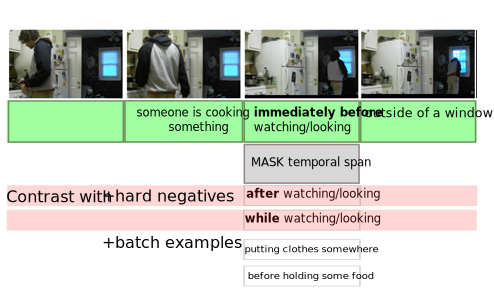
\includegraphics[width=1\textwidth]{cook}
	\caption{Example of an annotated instance, with a label across three
	segments. The middle segment contains a temporal word and is masked out.
	The contrastive span objective must identify the correct span out of the
	generated hard negatives and other batch spans. Note that audio and the
	other four segments are not shown here.}
	\label{fig:hard_neg}
\end{figure}


\section{Merlot Reserve Post-Pretraining}
\label{sec:training}

Using this dataset, we post-pretrain Merlot Reserve with a similar pre-training
objective and setup as described in~\citet{zellers2022mreserve}. We emphasise
the relevant points here.

\subsection{Architecture}
\label{ssec:arch}

We continue training on the Merlot Reserve Base model (+audio), which achieved
the highest downstream performance on STAR. The hyperparameters, unless
otherwise specified, are the same as Table 8 in~\citet{zellers2022mreserve}.
The image encoder is a 12-layer ViT-B/16
\acrlong{vit}~\citep{dosovitskiy2021vit}, which encodes each frame
independently.  Images are scaled to $192 \times 320$ with a patch size of 16.
Audio is encoded using an Audio Spectrogram Transformer~\citep{gong2021ast},
and we encode text spans into Byte Pair Encoding (BPE) tokens, using the same
embedding table as Merlot Reserve.  Differently to Merlot Reserve, we do not
split up audio and text encodings into subsegments, since the length of the
text spans in a segment are shorter in our dataset, and the average span length
per segment is close to the desired length of 5 tokens.

As in Merlot Reserve, the three modalities are combined in a joint encoder over
all input segments using a Transformer with 12 layers. Finally, a linear layer
of size 768 projects the output of the final layer's hidden state for
prediction of the masked segments. To learn the encodings of the targets for
each modality, the final hidden state of a \texttt{CLS} token is used for the
image and audio encoder, and a Transformer ``span encoder'' is learned to
extract text targets ``from a \texttt{CLS} [token] and embedded tokens of a candidate
text span''~\citep{zellers2022mreserve}. The overview from Merlot Reserve is
shown in~\cref{fig:mreservearch}.

\subsection{Objective Function}
\label{ssec:objective}

We use the contrastive span setup from Merlot Reserve, except we focus only on
learning temporal relations, as described in~\cref{ssec:contr_span}. The
objective function is therefore to minimise the cross-entropy between the
masked-out representation of the temporal segment $\mathbf{\hat{w}}_t$ and the
BPE encoding of the segment $\mathbf{w}_t$, along with encodings of spans from
the batch $\mathcal{W}$ and additional hard negative spans $\mathcal{W}_{hard}$, as described
in~\cref{ssec:neg_labels}. We do not include any masked audio segments.
The text span loss is therefore:
\begin{align}
	\label{eq:contrastive_loss}
	\mathcal{L}_{\mathrm{text}} = \frac{1}{( \mid\mathcal{W}\mid + \mid\mathcal{W}_{\mathrm{hard}}\mid )}
	\sum_{\mathbf{w}_t \in (\mathcal{W} \cup \mathcal{W}_{\mathrm{hard}})} 
	\left( \log	\frac{\exp(\mathbf{\hat{w}}_t \cdot \mathbf{w}_t)}
	{\sum_{\mathbf{w}\in(\mathcal{W}\cup\mathcal{W}_{\mathrm{hard}})} \exp(\mathbf{\hat{w}}_t \cdot \mathbf{w})} \right)
.\end{align}

We also include the frame-matching objective $\mathcal{L}_\mathrm{frame}$ from Merlot Reserve. The joint
encoder encodes the entire annotation, and we maximise similarity between the
\acrshort{vit} independent encoding of each frame to an extracted
representation from each segment. The loss function is the same
as~\cref{eq:contrastive_loss}, without the additional hard negatives $\mathcal{W}_{hard}$.
The complete loss function is the sum of both objectives:
\begin{align}
	\label{eq:total_loss}
	\mathcal{L} = \mathcal{L}_{\mathrm{text}} + \mathcal{L}_{\mathrm{frame}}
.\end{align}

We run our experiments on an NVIDIA GeForce RTX 3090 with a batch size of 8 for
up to 3 epochs. We use AdamW~\citep{loshchilov2019adamw} with the same
optimizer parameters as in Merlot Reserve, except we use a learning rate of
5e-6 after linear warmup over 3750 steps. The next chapter details the
downstream evaluation of this training process.
